\chapter{Background} \label{chapBackground}
\section{Application Areas}
We focus our efforts on two application areas: predicting carbon sequestration in forests and mapping vegetation types for forest fire mitigation. These provide representative examples to motivate vegetation type mapping and tree detection, respectively. 
\subsection{Forest Carbon Sequestration Prediction}
The first problem we explore is assessing carbon sequestration in forests. Forests are a massive sink of carbon, so protecting and managing our forests is a critical tool in the fight against climate change \cite{Griscom2017NaturalSolutions}. 
Clearing forests can result in substantial CO\textsubscript{2} emissions so it is especially important to keep existing forests intact. 
One tool to incentivize this is \textit{carbon credits}, which are payments to the landowner to keep carbon sequestered. These payments are often made by businesses or governments who have pledged to meet certain emission targets but cannot reduce their  CO\textsubscript{2} output to fulfill them immediately. Instead, they \textit{offset} these emissions by paying to have a commensurate amount of CO\textsubscript{2} emissions prevented. A key rationale for carbon credits is that some industries and activities are more challenging to de-carbonize than others, so it makes sense to direct funding toward the easiest solutions to achieve the largest near-term emission reductions. 
It is expected that demand for carbon credits will rise by a factor of 50 by 2050 according to Blaufelder et al. \cite{Blaufelder2021AChallenge}. 

%Unfortunately, there is widespread concern that carbon credits do not actually deliver the benefits that they promise. One issue is "additionality," which reflects the concern that a credit may be issued even when the business-as-usual outcome would not have resulted in releasing the carbon \cite{Gillenwater2011TheProgramme}. An example from forest-based carbon credits is when a landowner accepts payment for a carbon credit even though they did not intend to cut the trees if the credit had not been issued. Therefore, issuing the carbon credit did not actually have an impact on their behavior and therefore did not result in any less carbon being released.
%The second issue is that sequestered carbon can later be released. An example of this is forest fires burning trees that were used for carbon credits, thereby releasing CO\textsubscript{2} that was claimed to be sequestered \cite{Kaplan2023AccountingMarkets}. These two issues deserve rigorous and multi-disciplinary treatment to guarantee that carbon credits actually have the intended impacts. 
Unfortunately, there are many factors that make it challenging to guarantee that a forest-based carbon credit will have the desired impact and actually result in the claimed reduction in CO\textsubscript{2} emission. Some considerations are whether issuing the credit actually results in behavior change \cite{Gillenwater2011TheProgramme} or that carbon will later be released by uncontrollable factors such as wildfire \cite{Kaplan2023AccountingMarkets}. Another concern is that the established auditing approaches may overestimate the amount of carbon stored in a plot of land, which means that even in the best-case scenario, the desired amount of carbon sequestration is not being obtained. There are a variety of works showing that systematic over-crediting is common \cite{Badgley2022SystematicProgram,West2020OverstatedAmazon} due to biased modeling efforts or bias in human estimations. Technology can play a role in this area by improving upon simple regional models with empirical and site-specific information.

A common method for accurately estimating the carbon content of a forest is by taking a tree-centric approach. Each tree is located and the carbon content of each one is estimated individually. The per-tree carbon content can be regressed from phenotypic values such a basal (crown) area \cite{Torres2013UsingMexico} or predicted directly from images using machine learning \cite{Reiersen2022ReforesTree:Imagery}. The carbon content of the landscape can then be estimated by summing up the per-tree contributions. Our work on this topic focuses on the first stage of the carbon estimation process: detecting trees.

\subsection{Forest Fire Mitigation} 
\label{background:forest_fire_mitigation}
Destructive forest fires have increased dramatically over the past several decades \cite{spreading_like_wildfire, ayanz2021, nfn2022}. This is due in large part to climate change, which leads to hotter and drier weather along with stronger winds \cite{spreading_like_wildfire}. Climate change has also led to increased forest mortality from pests expanding their range, such as the mountain pine beetle in the Western US \cite{Jenkins2014AndFuels}. Humans have  contributed directly to fires by suppressing small fires which causes a build-up of flammable vegetation over time. Finally, there is an increase in ignition sources from careless human activity and infrastructure such as power lines. At the same time that fires are growing more common and destructive, more people live in close proximity to forests, furthering the risk of property loss, injury, and death. The ecological consequences of fire are also increasingly dire. Historical fires were a natural part of some ecosystems and vegetation was able to regenerate due to surviving trees and un-burned seeds. The intensity of modern fires destroys all vegetation and seeds, making it harder for regions to regrow. This can lead to erosion and eventual transition from forest to grassland.

It is becoming increasingly clear that reactive firefighting is insufficient to combat modern forest fires and preemptive mitigation efforts are also required \cite{spreading_like_wildfire}. One way to actively reduce the risk of destructive fires is by removing dense understory vegetation in a process termed fuel management \cite{Fire2021FuelsManagement, WildlandFireResiliencyProgram20214Plan, Agriculture2019HazardousComplex}. This is a challenging problem due to the sheer area of forested land and the limited resources currently put toward preemptive efforts \cite{spreading_like_wildfire}.

Fuel management is physically demanding and requires specialized knowledge, which has led to increasing concerns about labor shortages \cite{CommisionGlobalDivision}. 
%The threat of forest fires has driven increasing government interest in technological innovation, with the USDA \cite{USDA2023USDAGrant} and NASA \cite{SPSO2023Research2023} providing funding in this area. These grant opportunities address the need for pre-fire understanding and mitigation efforts rather than only reactive measures.
A recent robotics project proposed a multi-robot team that could autonomously remove vegetation \cite{couceiro2019semfire}. In their work, an unmanned ground vehicle can traverse the environment and mechanically grind vegetation, rendering it a less potent fuel source. This robot only has an understanding of its local environment, so the proposed concept relies on drones to map the environment beforehand. These drones determine both the geometric structure of the scene and the location of the fuel. This helps the robot avoid obstacles and determine where to go, respectively. Our work tackles this fuel mapping problem from the drone and proposes to extend this work to broader regions by predicting vegetation locations from remote sensing data. 


\section{Sources of Data for Forestry}
Most of our current forest understanding is at a broad scale \cite{Oswalt2014Update:}, but making intelligent forestry decisions requires granular information about the current state of the forest \cite{digitalForestry2009, Hogland2014EstimatingArcObjects}. The previous section highlights two examples where this is critical. Unfortunately, it is challenging to obtain information that is both accurate and covers a large enough region to inform management decisions at scale. We look at three sources of data that can inform forest management: observations from manual field work, images from small uncrewed aerial vehicles (UAVs or "drones"), and optical remote sensing data taken from aircraft or satellites. These three sources of data represent a trade-space between high interpretability from manual observations and high scalability from remote sensing.

\subsection{Manual Plot Measurements}
Understanding forests is still a largely manual process where foresters measure various quantities such as tree height, diameter, density, and species while in the field. In commercial contexts, this process is called a timber cruise \cite{ServiceFSHHANDBOOK} and in ecology, it is called a forest inventory \cite{USForestServiceDepartmentofAgriculture2016FORESTPLOTS}. Since this process is laborious, the established practice is to only take measurements at points or plots distributed throughout the environment \cite{Town2018ForestryMethods}. Choosing where to sample these plots is an important component of obtaining accurate and unbiased estimates for a region. Determining how to balance the size versus the number of plots and designing a sampling procedure both require substantial domain expertise. 

\subsection{Drone Surveys}
Drones equipped with cameras are increasingly used in forestry \cite{CristanDronesManagementEdited,Tang2015DronePractices}. This is driven by their comparatively low cost, ease of use, and flexibility. As described by Tang et al. \cite{Tang2015DronePractices}, drones fill a crucial operational gap by capturing higher-resolution data than crewed aircraft or satellites. Therefore, they are helpful for a wide variety of forestry tasks that require granular information.

Cameras are incorporated in nearly every drone because of their usefulness, low cost, and weight. Drones are often equipped with a commodity-grade GPS for navigation, which means that the captured images can be tagged with an approximate absolute location. Even though drones can be flown manually, it is common in forestry applications to use software such as QGroundControl \cite{QGroundControl} or DroneDeploy \cite{DroneDeploy} to plan a flight pattern. The user defines the perimeter of the area and sets parameters such as the survey pattern, altitude, and image density. The area that a drone can cover is often several acres but varies based on the type of drone and the type of flight plan. Similarly, the spatial resolution of the data varies but is on the order of centimeters per pixel.  While drones are a powerful tool, the raw data from them must generally be processed in a domain-specific manner to obtain the ecological information that is required by the end user.  

\subsection{Remote Sensing}
Remote sensing data is captured by sensors onboard satellites or airplanes and is rapidly becoming a critical tool for environmental monitoring \cite{Parra2022RemoteMonitoring}. This is largely because these sensors observe large---potentially global---regions and much of this data is available freely to the public. 
Remote sensing data can be from many modalities, such as light detection and ranging (LiDAR) \cite{LiDARForestryBeland2019}, synthetic aperture radar (SAR) \cite{Hall2020WhatEarthdata}, and electro-optical (EO) data.
In this work, we focus on electro-optical data, since it is prevalent and easy to interpret. This data is conceptually very similar to images taken by a traditional camera. While most consumer cameras only capture red-green-blue (RGB) information, remote sensing instruments often capture more distinct spectral bands, termed multi- or hyper-spectral data depending on the number. Another consideration is that remote sensing data often undergo many post-processing steps before being released. These include removing atmospheric effects, stitching images together, and re-sampling the data to lie on an axis-aligned grid. 
Optical remote sensing data has been used for numerous forestry applications such as mapping forest coverage \cite{ Hansen2013High-resolutionChange} and mapping forest type \cite{Kempeneers2011DataMapping}. Unfortunately, this technology has its limits, such as low spatial resolution which precludes granular analysis. For example, the forest extent mapping conducted by Hansen et al. \cite{Hansen2013High-resolutionChange} was only available at 30-meter resolution, because that was the resolution of the input data from the LandSat \cite{LandSat} satellite. This low resolution also means that multiple classes may be contained in one pixel, which further complicates automated analysis. 

\section{Interpreting Forestry Data}
The previous section highlights three types of data that can be obtained from forests. Manual forest inventories directly collect interpretable data, such as tree species and size, that can be statistically extrapolated to a larger region. The data from drones and remote sensing must be interpreted before it can be used to inform management decisions. As described in Section \ref{background:forest_fire_mitigation}, some applications require a detailed geometric understanding of the environment while others need a map of what type of vegetation is where.
%There are two primary insights we want to extract. The first is the purely geometric properties of the scene, e.g. a 3D map of the world. This can be used to inform the navigation of an autonomous robot. The second is semantic properties, such as what types of vegetation are where and the location and size of individual trees. 

\subsection{Understanding the Geometry of Scenes}
There are two approaches to understanding the geometry of forests that are common in a robotics context. The first approach, structure from motion, only requires a set of images about the scene but processing can only take place after the mission is complete. The second approach, simultaneous localization and mapping (SLAM), can be run online while the drone is flying, but often requires multiple complementary sensors for good results.
\subsubsection{Structure from Motion}
In general, commodity drones produce only monocular images with potentially a low-accuracy GPS and orientation estimate. A common approach for estimating geometry from this type of data is photogrammetry, also known as structure from motion or 3D reconstruction. Preliminary reconstructions of realistic large-scale scenes began with academic work such as \cite{Agarwal2009}. Over the last decade, numerous commercial and open sources software have been developed for this task, such as Agisoft Metashape \cite{AgisoftMetashape} and COLMAP \cite{schoenberger2016mvs, schoenberger2016sfm}, respectively.

The implementation details vary by application and assumption, but a common pipeline is the following: first, distinctive features are detected in each image. These represent small patches of pixels that are likely to be informative, such as corners and edges. Then, features are matched between images based on the local appearance. 
Given these corresponding points between images, multiple quantities can be estimated. The first is the location of these matched image points in the 3D space using triangulation between the cameras. The second is the location of the cameras. Finally, if the camera isn't accurately calibrated, it is common to estimate the \textit{intrinsic parameters} which describe how points in the world are projected onto the image. Given the interplay between all of these elements, it's critical to estimate them together in a global joint optimization. A widely-used class of techniques for solving this problem are termed bundle adjustment \cite{Triggs2000BundleSynthesis}. After the locations of the cameras have been estimated, it is possible to construct a dense point cloud or mesh representation of the scene, an example of which can be seen in Figure \ref{fig:background:camera_locations}.

Photogrammetry has been used in a variety of recent works on understanding forests \cite{Swayze2021InfluenceDensity, doi:10.1139/cjfr-2020-0433}. A notable work in this space is that of Young et. al. \cite{Young2022}. This work studies the impacts of different drone fight patterns and Metashape processing parameters on the quality of tree detection in complex coniferous forests. They analyze thousands of different configurations to propose a flight pattern and set of photogrammetry parameters that can be used in other tree detection applications.
\begin{figure}
    \centering
    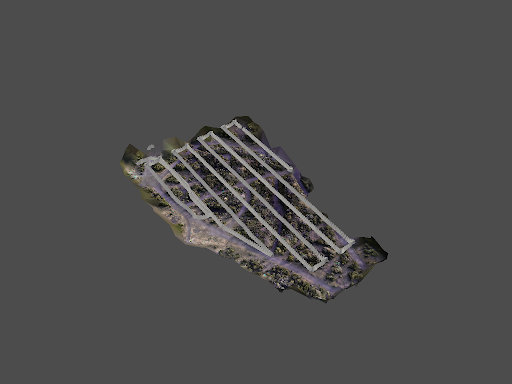
\includegraphics[width=0.8\textwidth, trim={4cm 3cm 4cm 4cm}, clip]{figs/methods/structure_from_motion/camera estimation.png}
    \caption{An example 3D reconstruction from Agisoft Metashape \cite{AgisoftMetashape} with the camera locations from the drone survey visualized.}
    \label{fig:background:camera_locations}
\end{figure}

%These solvers are becoming increasingly robust, and are well-suited to reconstructing scenes captured by drone surveys because the same location is often seen across many images.

\subsubsection{Simultaneous Localization and Mapping}
In settings where a drone is operating autonomously in complex environments such as under the canopy, it is important that it understands where it is in relation to obstacles in real time. This is necessary for the robot to can plan a trajectory and avoid collisions. The problem is known in robotics literature as simultaneous localization and mapping (SLAM) \cite{durrant2006simultaneous} since it involves solving two challenging problems at once. The first is localization, where the robot must determine its position within a known map. This is especially important in a forestry setting because GPS can be unreliable under forest canopies. The second is mapping, which involves building a 3D representation of the world using sensor data and the current location of the robot. In a new environment, the robot does not have a prior map, so these two interconnected tasks must be completed simultaneously.

In general, SLAM relies heavily on optimization approaches to jointly estimate the structure of the map and the location of the robot over time. Many modern approaches use factor graphs \cite{Dellaert2017FactorPerception}, which are an efficient formulation that allows previous estimates to be continuously refined as new information is obtained. A wide variety of SLAM systems have been proposed for different sensors and environmental settings. Many approaches use a LiDAR and an inertial measurement unit (IMU) because the former provides explicit 3D information and the latter provides an accurate estimate of the motion over a short time horizon even in uninformative environments. A commonly-used approach is LIO-SAM \cite{Shan2020LIO-SAM:Mapping}. This approach estimates the motion of the system by registering consecutive LiDAR scans, after using the IMU to remove distortion and provide an initial estimate to initialize the matching process. Another approach is LOAM \cite{Zhang2017}, which extracts geometric features such as corners and edges from the point LiDAR scans to provide more informative correspondences. This approach is more suitable for built environments than forests since these geometric features are less common in unstructured natural environments. However, an extension to LOAM, termed SLOAM \cite{Chen2020SLOAM:Inventory}, is designed specifically for forests. In SLOAM, they detect tree trunks from the LiDAR scans and use these trunks as landmarks to improve the localization. This approach shows strong results in forests but relies heavily on having a high-quality tree detection algorithm.

%A variety of generic SLAM approaches have been proposed in recent years for different combinations of sensors. One approach that uses a stereo camera is VIL-SLAM \cite{Shao2019StereoMapping}.
%such as LIO-SAM \cite{},  and LOAM \cite{Zhang2017}. These approaches are often primarily tested in urban or indoors environments and the work of Garforth et. al. \cite{Garforth2019VisualSLAM} explains some of the attributes that make forests difficult environments for vision-based SLAM.
%One work that proposes a forest-specific SLAM approach is SLOAM \cite{Chen2020SLOAM:Inventory}. This approach detects tree trunks and uses them as landmarks to increase the localization accuracy and robustness.

\subsection{Understanding the Content of Images}
Drones and remote sensing can collect a vast amount of data about the environment. Before this data is directly useful to land managers, it is important to extract quantities such as the location and size of trees or the types of vegetation in each region. Automated processing methods can free domain experts from the laborious task of interpreting data by hand. There has been a steady shift from methods that are hand-designed to those which learn from data. Supervised machine learning is a class of methods where the model is provided both the raw data and the correct interpretation.
The model that is developed from these training examples can be used to generate predictions on new data. Over the last decade there has been an explosion of approaches relying on deep learning \cite{Lecun2015DeepLearning}, which is a subset of machine learning using models with a large number of parameters that have multiple hierarchical processing steps. 
The parameters of these models are updated or \textit{trained} by an iterative process that seeks to minimize the error or \textit{loss} between the predictions and corrected labels. Because of the high number of parameters, these models often require large amounts of training data to generalize well to new data.

\subsubsection{Object Detection}
Object detection is the problem of identifying the location and shape of objects within an image. The shape of the object is often represented by an axis-aligned rectangle or a pixel-wise mask. These approaches can be trained to solely identify one type of object or identify and distinguish objects of multiple classes. In a forestry context, this could refer to both predicting the location and species of a tree. 

This problem has been extensively studied by the computer vision community over the last two decades. Early work was conducted by Dalal and Triggs \cite{Dalal2005humanDetection}, where they proposed a robust solution to pedestrian detection. Their approach leveraged well-engineered feature extraction using local changes in intensity and a support vector machine (SVM) classifier. Many approaches built on this concept, often still focusing heavily on extracting informative features from images. A seminal paper in 2012 by Krizhevsky et. al. \cite{NIPS2012_c399862d} showed that learning informative features from data using convolutional neural networks (CNNs) provided superior results to hand-crafted features on an image classification task. This sparked a trend of CNN-based object detection approaches. An early approach that is still commonly used today is Faster R-CNN \cite{Ren2017FasterNetworks}. This relies on a multi-stage approach, where the first stage predicts many rectangular candidate object locations. The second stage determines whether the proposal is indeed an object, predicts a refined bounding box, and optionally classifies the type of object. This approach was built upon by Mask R-CNN \cite{He2017MaskR-CNN}, which predicts a mask representing which pixels are part of the object instead of a rectangle. In contrast to the two-stage approaches, RetinaNet \cite{Lin2020FocalDetection} is an efficient single-stage approach that is especially suitable for dense objects, such as trees in a forest. In this work, the authors develop FocalLoss, a penalization strategy that focuses primarily on hard examples during network training.

\subsubsection{Semantic Segmentation}
Semantic segmentation is the task of assigning a classification label to every pixel in an image. In the forestry domain, these classes could be broad, such as trees, shrubs, and grasses, or more granular, such as different species of trees. An example image of this task can be seen in Figure \ref{fig:background:semantic_seg_example}.

\begin{figure}
    \centering
    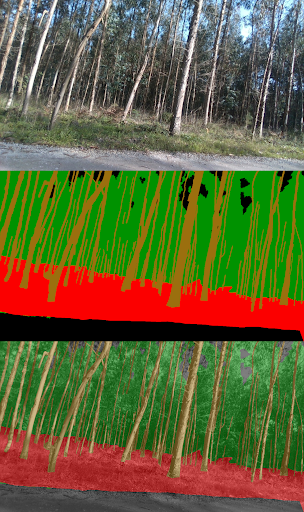
\includegraphics[width=0.45\textwidth, trim={0 340px 0 0}, clip]{figs/background/automated_understanding/segmentation_example.png}
    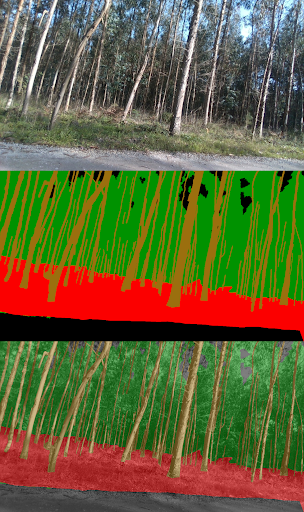
\includegraphics[width=0.45\textwidth, trim={0 170 0 170}, clip]{figs/background/automated_understanding/segmentation_example.png}
    \caption{A visualization of the goal of semantic segmentation. The input image is on the left, and the desired output is on the right, color-coded by class. Red is understory fuel, green is canopy, brown is trunk, and black is background such as bare earth and sky.}
    \label{fig:background:semantic_seg_example}
\end{figure}

An early work on semantic segmentation with deep learning was Fully Convolutional Network \cite{Shelhamer2017FullySegmentation}, which took early insights from image classification and adapted them to give per-pixel class predictions. Shortly following this was U-Net \cite{RonnebergerUNET2015}, which had an encoder-decoder architecture with skip connections to preserve high-resolution details. A wide variety of approaches have been developed since then, with slight variations on these initial concepts. There has been a recent shift toward using transformers \cite{Vaswani2017AttentionNeed} which has resulted in work such as SegFormer \cite{Xie2021} and SegNext \cite{Guo2022SegNeXt:Segmentation}. SegFormer is an especially compelling work because the authors conducted evaluations showing that the model generalizes well to data that looks different than what it was trained on. This is useful in the forestry context where there may be limited labeled data to train on and it is not fully representative of the entire scene. The goal behind SegNext is to provide the same level of performance as approaches such as SegFormer, but do so with less technical complexity and faster run-time. This is especially useful for performing semantic segmentation with limited computational resources, such as autonomous systems or laptops in the field.

\section{Summary}
This section summarizes the application areas for our work: forest fire mitigation, and carbon sequestration estimation. Both of these domains require accurate, granular, and scalable information about the state of the forest. We summarize the tradeoffs between data from manual field work, drone surveys, and remote sensing. Accurate---but small scale---information is provided directly by manual surveys, but drone and remote sensing data must be automatically processed to provide insights at scale. Two methods are common for understanding the geometric structure of the world from drone data: one that requires only simple sensors but requires offline processing and another that uses more complex sensors but can generate a map in real time. Deep learning has become a common tool for interpreting the content of scenes and is applicable for both vegetation segmentation tasks and individual tree detection. In this thesis, we use geometric reasoning to understand the structure of these scenes. We then train deep learning models for drone data using small amounts of ground truth information taken from the region and apply these models to the whole scene.